\chapter{Methodology used to refactor and improve RMT tool}%
\label{methodology}

This chapter explores the methodology for refactoring and improving the RMT tool. It delves into various techniques and best practices for improving and optimizing the tool's performance and maintainability. The discussion covers a range of refactoring strategies.

The methodology is delineated into five sequentially interconnected phases as depicted in \cref{fig-overview-methodology}. Each phase systematically uses the insights and understanding obtained from the previous stage to optimize its efficacy. 
\textcolor{red}{colocar na imagem e no texto seguintes os testes que fez com a RMT}.

\begin{figure}[ht!]
\SetCaptionWidth{\textwidth}
\caption{Methodology Overview Diagram}
\label{fig-overview-methodology}
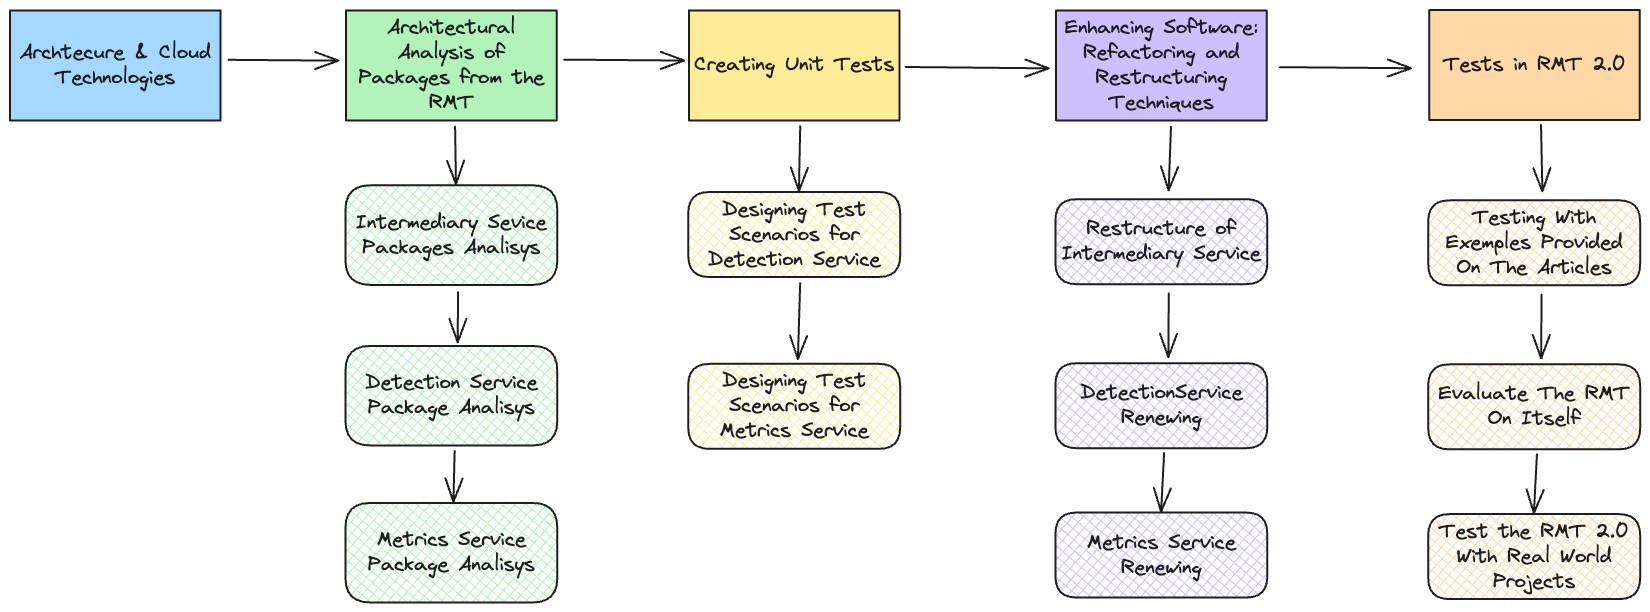
\includegraphics[width =\textwidth]{Chapter-4/Figures/Metodologia.png}
\SourceOrNote{Own authorship (2024)}
\end{figure}
\FloatBarrier


Each phase of the methodology is described in the clauses of this chapter. The \cref{sec-arch-cloud} explores the methodology through cloud technologies. The \cref{sec-archtectural-analysis}, \ref{sub-intermediary-packages}, \ref{sub-detection-packages}, and \ref{sub-metrics-packages} explain the analytic processes used to formulate strategic modifications to the codebase and delineate the functionalities of each package within the services. The \cref{sec-creating-tests}, \ref{detection-design-tests}, and \ref{metrics-design-tests} elaborate on the comprehensive testing procedures for each service, detailing the criteria for selecting tested classes. The \cref{sec-enhancing}, \ref{sub-restruct-intermediary}, \ref{sub-restruct-detection}, and \ref{sec-restruct-metrics} detail the extensive phases of refactoring and restructuring RMT services. The \cref{sec-test-rmt} outlines the systematic methodology implemented to evaluate the tool.

As all services have been renamed, the corresponding nomenclature equivalences are described in \cref{tab-services-map}. The explanations for the renaming are provided in the subsequent chapters.

\begin{table}[!ht]
    \centering
    \caption{Service names equivalency table}
\begin{tabular}{c c}
        \toprule
        \textbf{Original Name} & \textbf{New Name} \\
        \midrule
        Detection Service & Detection And Refactoring Service \\
        Metrics Service & Metrics Calculation Service \\
        Intermediary Service & Projects Sync BFF \\
        \bottomrule
    \end{tabular}
    \label{tab-services-map}
    \SourceOrNote{Own authorship (2024)}
\end{table}

\section{Archtecure \& Cloud Technologies}
\label{sec-arch-cloud}

The technologies selected for the revised architecture were thought to take greater advantage of what the cloud offers. 

Two technologies were selected for storage: the S3 Bucket from AWS and the Redis deployed as serverless with the Elasticache service. The S3 is a cheap object storage provided by AWS that is scalable and has a 99.9\% monthly uptime; it allows the tool to save zip files for each project and to be re-retrieved afterward \cite{S3}. The Redis is a widely used memory database for caching and allows us to easily save the project state \cite{Redis}.

The Simple Service Queue (SQS), a fully managed serverless queue service developed by AWS, was chosen for microservice communication. The SQS offers an async queue communication, having an order message delivered first in, first out (FIFO), or without an order \cite{sqs}.

Two services were selected for external communication: the Elastic Load Balancer (ELB) and the Amazon API Gateway. The ELB balances the load (requests) between services with a round-robin strategy \cite{Elb}. The API Gateway allows external communication to access the functionality for the back-end microservices \cite{Gateway}.


\section{Architectural Analysis of Packages from the RMT}
\label{sec-archtectural-analysis}

To understand the operational dynamics of RMT, it was imperative to analyze the codebase, specifically the various packages. The initial phase of the updating process involves discerning the functionality of different code segments to determine whether a code refactoring or a comprehensive service rewrite is necessary.

The analysis was carried out on the packages Intermediary Service, Detection Service, and Metrics Service, described below.

\subsection{Intermediary Sevice Packages Analisys}
\label{sub-intermediary-packages}
The intermediary service is systematically divided into four main packages, each comprising functionalities. The first functionality involves the management of refactoring projects. The second pertains to the facilitation of inter-service communication. The third serves as a service discovery mechanism by registering the addresses of all ancillary services to enable seamless subsequent communications. They are illustrated by the package diagram shown in \Cref{fig-package-intermediary}.

\begin{figure}[ht!]
\SetCaptionWidth{\textwidth}
\caption{Intermediary Service Package Diagram}
\label{fig-package-intermediary}
\includesvg{Chapter-4/Figures/intermediary-service.svg}
\SourceOrNote{Own authorship (2024)}
\end{figure}
\FloatBarrier

The package \texttt{datastore} includes configuration files relevant to the database pool and the connection configuration.

Package \texttt{files} contain repository files for database interactions, facilitating queries, insertions, and additional data manipulations.

Within the manager package, the entire outbound logic refers to the refactoring process and the discovery of services, encompassing all related requests for refactoring and generating metrics in the package \texttt{managers.projects} and registering services in the package \texttt{managers.members}.

For handling communication, the \texttt{ws.boundaries} package includes the controller configurations. Within this package, business logic is assigned to the persistence and querying of projects and dispatching requests to other services. Consequently, this package must access the \texttt{managers} and \texttt{files} packages.

\subsection{Detection Service Package Analisys}
\label{sub-detection-packages}

The detection service is arranged into six main packages, the core functionalities of which are periodically communicated with the intermediary service to ensure registration with the service discovery mechanism. In addition, interfaces have been developed to analyze the source code for potential refactoring candidates, and interfaces have been designed to perform refactoring on projects that contain such candidates. The package diagram displayed in \Cref{fig-package-detection} illustrates them.
\begin{figure}[ht!]
\SetCaptionWidth{\textwidth}
\caption{Detection Service Package Diagram}
\label{fig-package-detection}
\fontsize{7.5}{9.5}\selectfont
\includesvg[width =\textwidth]{Chapter-4/Figures/detection-service.svg}
\SourceOrNote{Own authorship (2024)}
\end{figure}
\FloatBarrier

The package \texttt{datastore} is configured with identical database parameters to those defined in \cref{sub-intermediary-packages}.

Package \texttt{ repository.project} has logic to manipulate the database where projects are saved and retrieved for unrefactored and refactored projects. The database configuration, such as the address and ports, is imported from the \texttt{datastore} package.

The package \texttt{methos.dataExtractoins} includes preconfigured interfaces for implementing various code extraction methods. The Abstract Syntax Tree is implemented as the extraction method for the refactoring processes within the RMT. Following the code transformation into an Abstract Syntax Tree (AST), the service accesses the files within the \texttt{domain.mehtos} to perform its designated function.

The package \texttt{managers.pulse} includes the configuration for the service registry, sending requests every minute to ensure its functionality to the intermediary service, and can receive requests. Information, such as the address and port sent from the service, is retrieved from the package \texttt{domain.identity}.

The interfaces for candidates searching and refactoring projects are in the \texttt{domain.methdos} has interfaces to implement and extend the tool refactoring options. As the current methods implement the Abstract Syntax Tree as an extraction method, the \texttt{doamin.dataExtraction.utils} package has methods to facilitate AST manipulation.

To start refactoring, the controllers must receive an HTTP request on the \texttt{ws.boundaries} that distributes the request based on its URL path among the other class functions. 

\subsection{Metrics Service Package Analisys}
\label{sub-metrics-packages}

The metrics service is divided into six main packages and two main functionalities; as the detection service, the metrics service communicates with the intermediary service for the service registry; the second functionality calculates metrics and quality attributes (calculated with the metrics results). The services have interfaces to increase the available metrics and quality attributes. The \cref{fig-package-metrics} shows the diaram package.

\begin{figure}[ht!]
\SetCaptionWidth{\textwidth}
\caption{Metrics Service Package Diagram}
\label{fig-package-metrics}
\fontsize{9}{10}\selectfont
\includesvg[width =\textwidth]{Chapter-4/Figures/metrics-service.svg}
\SourceOrNote{Own authorship (2024)}
\end{figure}
\FloatBarrier

Consistent with the two preceding services, the \texttt{ datastore} is the repository for all database configuration settings.

To access the unrefactored and refactored projects, the package \texttt{repository.project} has all the logic queries to the database using the information provided by the \texttt{datastore} package.

Correspondingly to the previous service, the package \texttt{managers.pulse} encompasses the comprehensive logic required for registration within the service discovery mechanism. This service adheres stringently to all the specifications delineated in the detection service.

Similarly to the detection service, the \texttt{processor.qualityAttributes} has the interfaces to implement different methods of measuring code metrics and quality attributes. The interfaces' logic and calculations are in the \texttt{domain.metrics} and \texttt{domain.qualityAttribute} packages.

The classes with logic and calculations for generating metrics are in the \texttt{domain.metrics} package; for now, they are hardcoded, implementing the CK module created by \textcite{ck}; however, the interface is designed to integrate additional metrics generation methodologies in the \texttt{domain.qualityAttributes} package is located in the calculations for quality attributes, such as maintainability, readability, etc.

Consistent with previous services, the \texttt{ws.boundaries} packages serve as the access point for service functionalities. They coordinate computations by interfacing with the database to retrieve project data and invoke methods within the \texttt{processor.qualityAttributes} packages, thereby generating metrics and quality attributes.
 
\section{Creating Unit Tests}
\label{sec-creating-tests}

Upon comprehending the tool's functionalities, the subsequent step involves verifying the presence of tests. This is essential to commence the refactoring process, as explained by Fowler:

\Citation[english]{\cite[9]{fowler2018refactoring}}{Whenever I do refactoring, the first step is always the same. I need to ensure I have a solid set of tests for that section of code. The tests are essential because even though I will follow refactorings structured to avoid most of the opportunities for introducing bugs, I’m still human and still make mistakes}.

The RMT lacked any form of testing; therefore, according to \textcite{fowler2018refactoring} philosophy, the tool was subjected to unit tests to verify consistent behavior after refactoring. 

The tests focused on the business logic of the detection service and the quality attribute computations within the metrics service. Testing was bypassed for the intermediary service due to its redevelopment.

The tests were designed exclusively for classes with specific logic, excluding interfaces, enumerations (enums), and Plain Old Java Objects (POJOs). This exclusion is justified, as such classes only exhibit the intrinsic behavior provided by the programming language itself without incorporating any additional logic. Consequently, there is no need to test these classes.

\subsection{Designing Test Scenarios for Detection Service}
\label{detection-design-tests}

Tracing the tool's execution path, the initial classes slated for testing are within the \texttt{methods} package, as they are the classes responsible for parsing the code into an Abstract Syntax Tree (AST). 

After refactoring, the parsing behavior must remain consistent, given that the AST is the foundational structure enabling the tool's capacity to manipulate Java classes to refactor. The \cref{fig-class-detection-methods} illustrates the simplified class diagram for the Methods package.

\begin{figure}[ht!]
\SetCaptionWidth{\textwidth}
\caption{Detection Service Methods Package Simplified Class Diagram}
\label{fig-class-detection-methods}
\fontsize{7}{8}\selectfont
\includesvg[width =\textwidth, scale=1.0]{Chapter-4/Figures/detection-service-methods.svg}
\SourceOrNote{Own authorship (2024)}
\end{figure}
\FloatBarrier

The initial phase of the RMT refactoring process, 'data extraction,' involves parsing Java files into an Abstract Syntax Tree (AST), a task performed by the \texttt{AbstractSyntaxTree} class. The class testing methodology consists of the accuracy of the parsing process, the generation of an AST object, or the identification of errors as the library \cite{javaparser} executes the process. Therefore, the reliability of this library is assumed, necessitating only the validation of the output. This is achieved by converting a code sample into a string and confirming the equivalence between the AST output, also as a string, and the original input. Error conditions are tested by deliberately invoking the library with incorrect Java code and asserting the results.

The \texttt{AbstractSyntaxTreeFork} class orchestrates the refactoring implemented methods that use the Abstract Syntax Tree (AST) as the parsing mechanism. The refactoring process is divided into two primary stages: invoking methods to identify candidate elements and executing methods to refactor the identified candidate classes. Additionally, the class has logic for database manipulation; this aspect was not subjected to testing due to the substitution of all database communication mechanisms and the database itself, thereby preventing the necessity to preserve any pre-existing behavior. For testing the class, the refactoring techniques had to be mocked (creating an object that simulates the original object's behavior) and assuring the behavior when the methods return an error or success.

The \texttt{DetectionMethodsManagerImpl} was excluded from the testing due to the planned complete reimplementation of the class, which encapsulates the algorithms for project retrieval from the database and the execution of procedures within \texttt{AbstractSyntaxTreeFork}.

The methods executed by \texttt{AbstractSyntaxTree} are situated within the \texttt{methods} package and hold the logic for each implemented refactoring method. The classes are split into two distinct categories: the first category contains classes designed to identify refactoring candidates by detecting specific patterns within Java code that qualify for refactoring; the second category consists of classes intended to execute the refactoring process, thereby effectuating the requisite modifications to the code. The simplified class diagram is divided into two \cref{fig-class-detection-domain-wei} and \cref{fig-class-detection-domain-zafeiris} representing these classes.

\begin{figure}[ht!]
\SetCaptionWidth{\textwidth}
\caption{Detection Service Domain Package Simplified Class Diagram For Wei Related Files}
\label{fig-class-detection-domain-wei}
\fontsize{4}{5}\selectfont
\includesvg[width =\textwidth]{Chapter-4/Figures/detection-service-domain-wei.svg}
\SourceOrNote{Own authorship (2024)}
\end{figure}
\FloatBarrier

The \cref{fig-class-detection-domain-wei} illustrates the class diagram for the \cite{liu2014automated} method, whereas the \cref{fig-class-detection-domain-zafeiris} outlines the class diagram for \cite{zafeiris2017automated} method.

\begin{figure}[ht!]
\SetCaptionWidth{\textwidth}
\caption{Detection Service Domain Package Simplified Class Diagram For Zafeiris Related Files}
\label{fig-class-detection-domain-zafeiris}
\fontsize{5}{8}\selectfont
\includesvg[width =\textwidth]{Chapter-4/Figures/detection-service-domain-zafeiris.svg}
\SourceOrNote{Own authorship (2024)}
\end{figure}
\FloatBarrier

The classes \texttt{WeiEtAl2014Candidate}, \texttt{WeiEtAl2014FactoryCandidate}, \texttt{ZafeirisEtAl2016Candidate}, and \texttt{WeiEtAl2014StrategyCandidate} were excluded from testing, as previously mentioned since Plain Old Java Objects (POJOs) devoid of any business logic were not subjected to testing. The \texttt{WeiEtAl2014} and \texttt{ZafeirisEtAl2016} classes were also excluded from testing as they had been rewritten.

The initial tested class was the \texttt{AstHandler}, serving as an encapsulating wrapper that facilitates direct access to an AST branch. The test cases must ensure that the methods can access the AST objects, such as methods, variables, inner classes, etc. The class also has some methods with limited logic, like assuring that two variables are the same and finding a class's parent, among others. Those functionalities were tested to ensure that they worked as intended and would continue after the refactoring. Some opportunities for improvement were discovered during the development of test cases, which are addressed in \cref{results}. 

The tests for the following classes are categorized into two distinct groups: verifiers and preconditions and executors. The preliminary classes subjected to testing were related to the \textcite{liu2014automated} methods, specifically \texttt{WeiEtAl2014FactoryVerifier}, \texttt{WeiEtAl2014StrategyVerifier}, and 	\texttt{WeiEtAl2014StrategyVerifier} and \texttt{LiteralValueExtractor}. It is intrinsic to the verifier to have methods that return a boolean, so the test must ensure that the method returns true if the case has the right condition and returns false if it is wrong. Under the analogous implementation approach brought about by the \textcite{zafeiris2017automated} method, the subsequent classes, namely, \texttt{ZafeirisEtAl2016Verifier}, \texttt{ExtractMethodPreconditions}, \texttt{SiblingPreconditions}, and \texttt{SuperInvocationPreconditions}, were subjected to identical rigorous tests.

The following tests targeted executors in both refactoring methods, beginning again with the paper by \textcite{liu2014automated} with specific classes tested included \texttt{WeiEtAl2014FactoryExecutor} and \texttt{WeiEtAl2014StrategyExecutor}; concerning the 	\textcite{zafeiris2017automated} article, the scrutinized class was \texttt{ZafeirisEtAl2016Executor}. The testing methodology for these executors is straightforward; within each referenced publication, the authors illustrate the functionality of the refactoring approaches by providing authentic code exemplars. These examples were used to verify that the output generated by the executors corresponded precisely to the outputs delineated in the respective papers.

\subsection{Designing Test Scenarios for Metrics Service}
\label{metrics-design-tests}

Most classes within the Metrics services require extensive rewrites to integrate the new architectural framework. Consequently, testing was limited to only three classes represented in \cref{fig-class-metrics-quality}, excluding \texttt{QualityAttributeMetric} because it is a POJO.

\begin{figure}[ht!]
\SetCaptionWidth{\textwidth}
\caption{Metrics Service Simplified Class Diagram for Tested Classes}
\label{fig-class-metrics-quality}
\includesvg{Chapter-4/Figures/metrics-service-quality-attributes.svg}
\SourceOrNote{Own authorship (2024)}
\end{figure}
\FloatBarrier

The critical aspect of testing metrics and quality attributes for refactoring lies in maintaining consistent calculations for metrics and quality attributes. This ensures that the test's integrity remains intact, notwithstanding any alterations in the library that may modify the metric computation method.

Performing an in-depth analysis for each class. The \texttt{Metric} class extracts metrics from the \textcite{ck} library, incorporating these metrics for each class within a project. The test must ensure the continuity of the metric calculations for each class using identical metrics derived from the CK library. The \texttt{Proportion} class encompasses two calculation methodologies: the \texttt{direct} method, entailing the division of the refactored value by the original, and the \texttt{inverted} method, which involves the division of the original value by the refactored; testing must ensure that these calculations yield consistent results after refactoring. The \texttt{QualityAttribute} class served as the foundational model to calculate the quality attributes used in RMT. This was achieved by integrating the results of specific metrics with proportion calculations; the testing process must confirm that identical metric values consistently yield the same quality attribute values, even after subsequent refactoring.

\section{Enhancing Software: Refactoring and Restructuring Techniques}
\label{sec-enhancing}

After creating tests, the tool can be refactored and restructured. The first step in refactoring the RMT was to update the Java version to 21 since the current version was 8, released in 2014; the new version brings new features to the language and is faster \cite{java21}. 

Despite the advantages of upgrading the Java JDK, one of the fundamental tenets of the refactoring initiative was to transition the framework to Spring Boot. Consequently, since the latest version of Spring Boot is exclusively compatible with Java 17 and higher. All dependencies were also updated to the latest version.

IntelliJ, developed by JetBrains, was the integrated development environment (IDE) for refactoring the tool \cite{intellij}. IntelliJ has an "inspection" functionality that proactively recommends refactorings of the current code, with the primary objective of enhancing it \cite{intellij-inspection}. In the RMT code, suggestions were made to make the code more readable, such as changing an expression from a negated to a regular expression, as exemplified in \cref{alg-intellij}. The IntelliJ automation subjected the metrics and detection services to a comprehensive refactoring process.

\begin{algorithm}[!htbp]
\caption{Exemple of a code refactoring by IntelliJ}%
\label{alg-intellij}
\begin{algorithmic}[1]
\STATE{var a = Optional.ofNullable(variable)}
\STATE{if(!a.isPresent()) \{...\}} \COMMENT{Exemple of code IntelliJ highlights to refactor}
\STATE{if(a.isEmpty()) \{...\}} \COMMENT{Code after refactoring}
\end{algorithmic}
\SourceOrNote{Own Authorship (2024)}
\end{algorithm}
\FloatBarrier

The Spring Framework was integrated into the detection and metrics services to initiate the early refactoring. Concurrently, all dependencies associated with the legacy database, including files specific to its utilization, were removed. The prescribed method for framework application began with the controllers (even though they would be removed afterward) and subsequently extended to the imported classes. It was not requisite for all classes to undergo modifications to align with the refactoring; however, classes exhibiting ambiguous behavior were earmarked for subsequent review during the functionality improvement phase. The tool was no longer functional, but previously implemented tests backed its functionality.

The sequence for restructuring the tool begins with the complete rewrite of the intermediary service, as it is the only service that receives requests from the user following the new architecture. Refactoring progresses to the detection service as it gets the message sent by the intermediary service, processes it, and sends it to the metrics service if any candidate is found. The process is complete in the metrics service, which is the last service in the architecture.


%Iniciei tentando adiconar coisas de novas versões do Java pro codigo ficar mais limpo e atualizar a dependencias.
%Refatorei de acordo com as dicas do intellij.
%Adicionar o novo framework nos 2 serviços.
%Explicar por qual modulo comecei a refatorar e porque. Durante a refatoração do modulo confrome as funcionalidades foram implementadas para aperfeiçoa-las os pacotes e classes necessarios foram sendo criados.

%Pegar as limitacoes e explicar como elas foram refatoradas
\subsection{Restructure of Intermediary Service}
\label{sub-restruct-intermediary}

As previously mentioned, the intermediary service underwent a comprehensive restructuring due to the obsolescence of most of its functionalities according to the new design. 

The remaining essential features were also rewritten but updated to integrate current technologies. The rewrite addresses some limitations of the RMT by focusing on keeping the service simple implementation and the asynchronous management of the tool. The intermediary service is assigned to receive a project via HTTP, save the project information in the event database, the project file on an object storage tool, send the project ID to the detection service and close the requests successfully. The tool also offers an endpoint to consult the refactoring status, as the process is asynchronous.

Those modifications attempt to solve the service freezing issue and remove many responsibilities from it. The freezing is avoided because the service is ready to receive a new request after sending a message to the detection service without waiting for the service process to respond. Concerning responsibilities, the service does not have a load balancer or a service registry functionality, which helps to save machine resources.

As the tool is no longer an intermediary service, the name was changed to Project Sync BFF (back-end for front-end). The name implies that the service offers APIs to sync the project and, therefore, an endpoint to register the project and others to verify the project status. The service also provides an endpoint that creates a zip file with the chosen refactorings and returns a link to download them.

%Mudei o nome e justicar. 
%Mudei a formal de funcionamento e porque

\subsection{Detection Service Renewing}
\label{sub-restruct-detection}

The detection service refactoring began with replacing and removing obsolete files, including substituting the controller with a queue consumer and replacing previously deleted database files with new ones, contemplating the new architecture technologies. Following the replacement of the controllers and the integration of the new database access files, the effort to address the service limitations began.

The main limitation of the service was the disk access problems, in which a refactoring would access the disk many times to save and parse the files again. To address the problem, a new object was created to store the files to be used solely in memory. While replacing old objects, some optimizations in memory usage and performance were performed by removing duplicate codes and only parsing the Java files once for each refactoring method.

The name was changed from the detection service to the detection and refactoring service as it detects candidates and refactors.


%Erros econtrados nos testes

\subsection{Metrics Service Renewing}
\label{sec-restruct-metrics}

Refactoring started as in the last service, in the service metrics, by replacing the controller with a queue consumer and the database repository files with the new ones. As a known limitation, the CK library \textcite{ck} was removed from hard-coded as a Maven dependency to facilitate management and updates. 

The service also had some logic for the metrics and quality attributes implemented in Enums; this logic was reimplemented in a strategy pattern and improved by calculating the metrics only once for each candidate instead of three times as in the previous code.

Following the other two services, the name was also changed from metrics service to metrics calculation service as it is a more meaningful name. 

%Removi a CK que estava no codigo, atualizei e importer via package manager
%adicionei novos padrões

\section{Tests in RMT 2.0}
\label{sec-test-rmt}

Despite the presence of unit tests following the refactoring process, the tool has undergone system-level testing. A Dockerfile was generated for each service to establish the integration test environment, which allows containerization. To facilitate the local execution of AWS services, Localstack \cite{localstack} enables SQS and S3 services, with Redis provisioned in a separate container. The deployment of all these containers is orchestrated using a docker-compose file. 

The evaluation of the tools was systematically organized into three sequential phases. The initial phase involved validating the examples presented in the works of \textcite{liu2014automated} and \cite{zafeiris2017automated}. Subsequently, an analysis of the RMT by itself was performed, which included versions 1.0 and 2.0. The final phase comprised testing the tool using the equivalent, updated projects that were utilized in the evaluation of the tool's first version. The results of the three testing phases are presented in the next chapter.

\section{Cloasing Remarks}

This chapter presented the methodology used to improve and refactor the RMT tool. 
The methodology outlined is sketched through the diagram described \cref{fig-summarized-methodology}. It is partitioned into six distinct color segments to enhance the elucidation of the process, which starts with improving the RMT and follows a path to every step in the methodology until the tool is refactored and ready to be tested.

\begin{figure}[ht!]
\SetCaptionWidth{\textwidth}
\caption{Diagram summarizing the improvement methodology}
\label{fig-summarized-methodology}
\fontsize{3.8}{5}\selectfont
\includesvg[width =\textwidth]{Chapter-4/Figures/methodology-mind-map.svg}
\SourceOrNote{Own authorship (2024)}
\end{figure}
\FloatBarrier

The green nodes represent the analyzed service process. The pink nodes indicate the processes associated with the restructuring of the architecture and the creation of tests. The yellow nodes are for the service refactoring process. The purple nodes designate the testing phase of the implemented changes, while the orange nodes correspond to the correction of identified issues.

\textcolor{red}{tem que explicar em alto nível a image 17}